\filbreak
\Rank{A問題}

\Mon{基本公式の確認}

% 再編：原本 第24回［41］（屈折の4小問）と 第25回［45］（回折格子1小問）を1題に統合した．
\hspace{1zw}真空中の光速を$c=3.0\times 10^8\U{m/s}$として，以下の設問に答えよ．ただし，空気の絶対屈折率は1とする．
\begin{komon}
\ko{1} 絶対屈折率1.5のガラス中を進む光の速さは何$\U{m/s}$か．
\ko{2} 光が真空中からある物質に入射角$60^\circ$で入射したところ，屈折角は$30^\circ$であった．この物質の絶対屈折率を求めよ．
\ko{3} 絶対屈折率がそれぞれ1.5, 2.0のガラス\MARU{1}，\MARU{2}がある．ガラス\MARU{1}に対するガラス\MARU{2}の相対屈折率を求めよ．
\ko{4} 絶対屈折率2.0の物質から真空中へ光が進むときの臨界角を求めよ．
\ko{5} 回折格子に対して垂直に波長$600\U{nm}$の単色光を当てたところ，入射方向に対して$30^\circ$の方向に1次の明線が生じた．この回折格子$1\U{m}$あたりの格子の本数は何本か．
\end{komon}

\filbreak
\Rank{B問題}

\Mon{波の性質}

\hspace{1zw}次の文の\fbox{\phantom{\MARU{0}}}内に当てはまる適当な語句を答えよ．

\hspace{1zw}波が伝わって行くとき，ある瞬間の波面$\mathrm{AB}$上の各点を中心として\fbox{\MARU{1}}とよばれる2次的な\fbox{\MARU{2}}波が無数にでき，これらによって次の瞬間の新たな波面$\mathrm{A}^\prime\mathrm{B}^\prime$ができる．新たな波面$\mathrm{A}^\prime\mathrm{B}^\prime$はこれらの無数の\fbox{\MARU{1}}のすべてに接する曲面（すなわち包絡面）となっており，これを\fbox{\MARU{3}}の原理という．

\hspace{1zw}また波が障害物の背後に回り込んで伝わる現象を\fbox{\MARU{4}}といい，障害物のすき間の幅が波の\fbox{\MARU{5}}と同じかそれ以下になると，この現象が著しくなる．そのため，通常の日常生活においては，音波と光波（可視光）では\fbox{\MARU{6}}の方が\fbox{\MARU{4}}の現象を起こしやすい．

\Mon[\Sitei]{屈折の法則}

\begin{zuright}{62mm}
\hspace{1zw}右の図のように媒質$\mathrm{A}$, $\mathrm{B}$が重なっており，これが真空中に置かれている．媒質$\mathrm{B}$の内側から，媒質$\mathrm{A}$, $\mathrm{B}$の境界面に向けて入射角$30^\circ$で光を入射させたところ，光は図のように屈折して真空中へと抜けていった．真空中での光の速さを$3.0\times 10^8\U{m/s}$として，以下の設問に答えよ．
\zusep
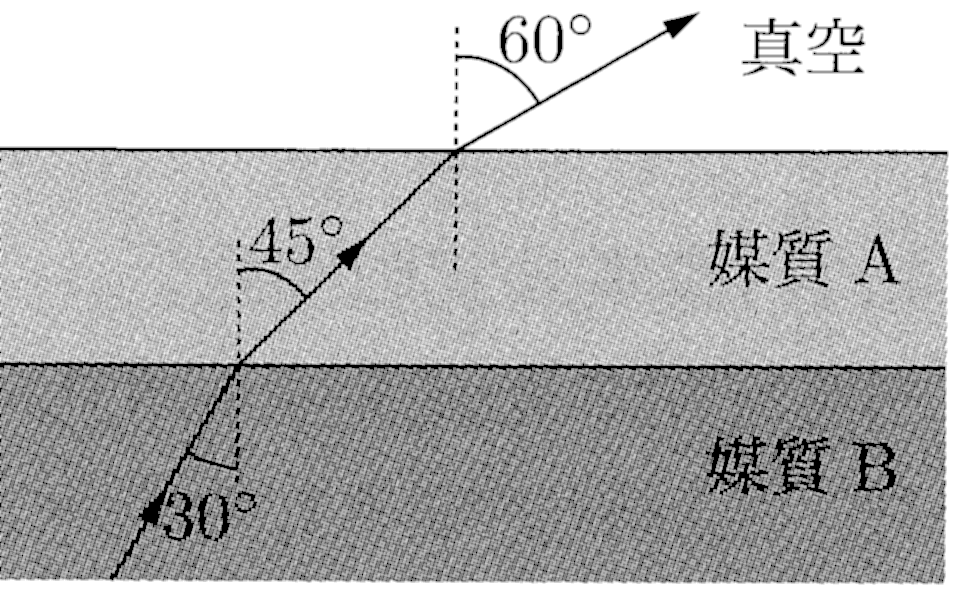
\includegraphics[keepaspectratio,width=62mm]{fig/ch18_ex_refract.png}
\end{zuright}
\begin{komon}
\ko{1} 図を元に，媒質$\mathrm{A}$, $\mathrm{B}$の絶対屈折率$n_\mathrm{A}$, $n_\mathrm{B}$を求めよ．
\ko{2} 媒質$\mathrm{B}$中での光の速さを求めよ．
\ko{3} 光が媒質$\mathrm{A}$と真空との境界面ですべて反射されて全反射になるためには，媒質$\mathrm{B}$の内側から媒質$\mathrm{A}$, $\mathrm{B}$の境界面に進む入射光の入射角の正弦の値がどのような範囲になければならないか．
\end{komon}

\Mon{水中の光源を隠す円板の半径}

\begin{zuright}{62mm}
\hspace{1zw}水面から深さ$h\U{m}$の位置に点光源$\mathrm{P}$がある．水面に円板を浮かべて，空気中のどこから見てもこの光源が見えないようにするためには少なくともどれだけの半径の円板を浮かべればよいかを考える．空気に対する水の相対屈折率を$n$として，以下の設問に答えよ．
\zusep
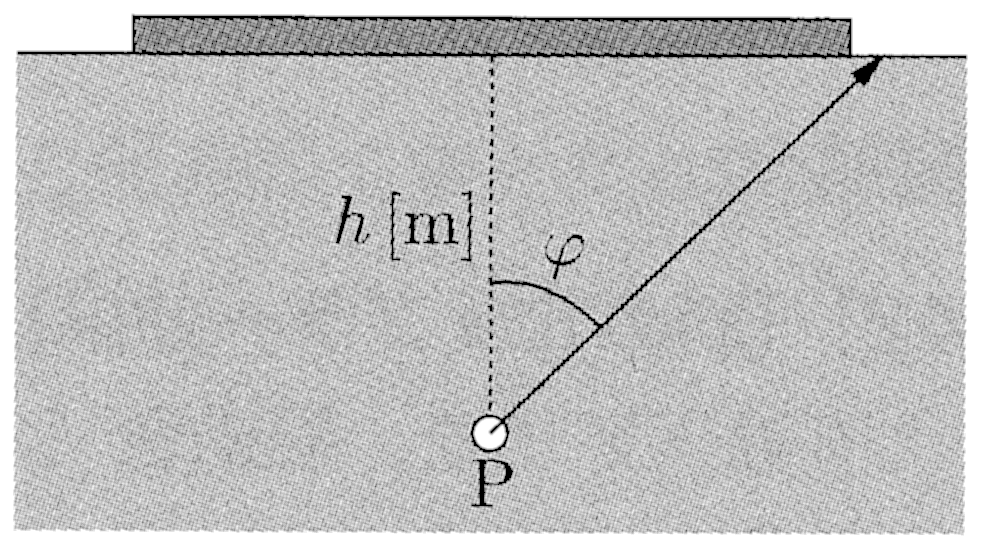
\includegraphics[keepaspectratio,width=62mm]{fig/ch18_p45_disk.png}
\end{zuright}
\begin{komon}
\ko{1} 光源$\mathrm{P}$から図のような角度$\varphi$の方向に出た光が，水面で全反射するために必要な$\varphi$に関する条件式を導け．
\ko{2} 円板の半径の最小値$R_0\U{m}$を求めよ．
\end{komon}

\Mon{光ファイバーの原理}

\begin{zuright}{68mm}
\hspace{1zw}右図のように，透明な絶対屈折率$n_1$の物質\MARU{1}で円柱を作り，その円柱\MARU{1}の側面を絶対屈折率が$n_2$の被覆材\MARU{2}で覆ってケーブルを作る．このケーブルが光ファイバーケーブルとして利用できるためにはどのような条件が必要かを考えてみよう．これを空気中に置いて利用するものとして以下の設問に答えよ．ただし$n_1>n_2$であるとし，空気の絶対屈折率は1であるとする．
\zusep
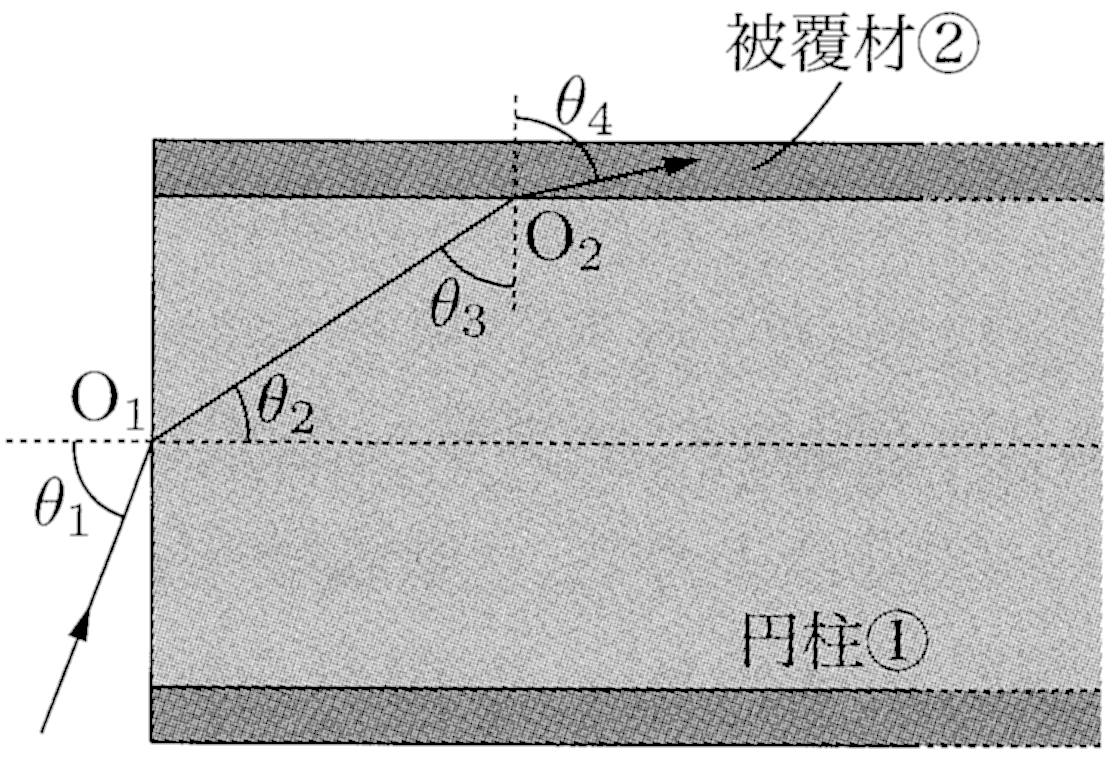
\includegraphics[keepaspectratio,width=68mm]{fig/ch18_p46_fiber.png}
\end{zuright}
\begin{komon}
\ko{1} 円柱の端面の点$\mathrm{O_1}$に外部から光が入射角$\theta_1$で入射し，これが屈折角$\theta_2$で屈折したとする．このとき$\theta_1$, $\theta_2$の間に成り立つ関係式を示せ．
\ko{2} (1)の屈折光が被覆材との境の点$\mathrm{O_2}$に達し，被覆材内部へ屈折角$\theta_4$で屈折していったとする．$\mathrm{O_2}$点への入射角を$\theta_3$とするとき，$\theta_3$, $\theta_4$の間に成り立つ関係式を求めよ．
\ko{3} 以上より，$\theta_1$, $\theta_4$の間に成り立つ関係式を求めよ．
\ko{4} 円柱の端面の点$\mathrm{O_1}$に対して図のような入射角$\theta_1$で入射した光がケーブル内（円柱\MARU{1}内）で反射を繰り返して伝わっていくために必要な，$n_1$に関する条件式を求めよ．
\ko{5} このケーブルを光ファイバーケーブルとして利用するためには，円柱\MARU{1}の側面から入射したすべての光が反射を繰り返して伝わっていくことが必要である．このために必要な，$n_1$, $n_2$の間の条件式を示せ．
\end{komon}
